\documentclass{exam}

\usepackage{amsmath,amssymb,amsfonts,amsthm,dsfont}
\usepackage{lib/extra}
\usepackage{graphicx}
\usepackage{tikz}
\usepackage{enumitem}
\usepackage{bbm}
\usepackage{pgfplots}
\usepackage{fontenc}
\usepackage{float}

\usepackage{subcaption}

\pgfplotsset{compat=1.18}

\title{ECE 569 HW 3}
\author{Brandyn Tucknott}
\date{Due 5 December 2025}

\begin{document}
\maketitle


All code has been submitted on canvas.
\begin{questions}
    % question 1
    \question Consider the classification problem in HW 2. Implement the following using CVX.
    \begin{parts}
        % question 1.a
        \part Apply the C-Hull formulation to train a classifier:
        \begin{align*}
            \MIN{u, v} & ||Au - Bv ||_2^2 \\
            \subjectto & 1^Tu = 1, u \succeq 0 \\
            & 1^Tv = 1, v \succeq 0.
        \end{align*}
        Visualize the training data together with a classifier. Also visualize the testing data and the classifier in another figure,
        and report the classification error on the testing data using the true labels provided in \qcr{test\_separable.mat}.
        \begin{figure}[H]
            \centering

            \begin{subfigure}[b]{0.48\textwidth}
                \centering
                \includegraphics[width=\textwidth]{figures/school_work/ECE_569/HW_3/c-hull-separable-train.eps}
                \caption*{Figure 1: C-Hull Classifier, Separable Training Data}
            \end{subfigure}
            \hfill
            \begin{subfigure}[b]{0.48\textwidth}
                \centering
                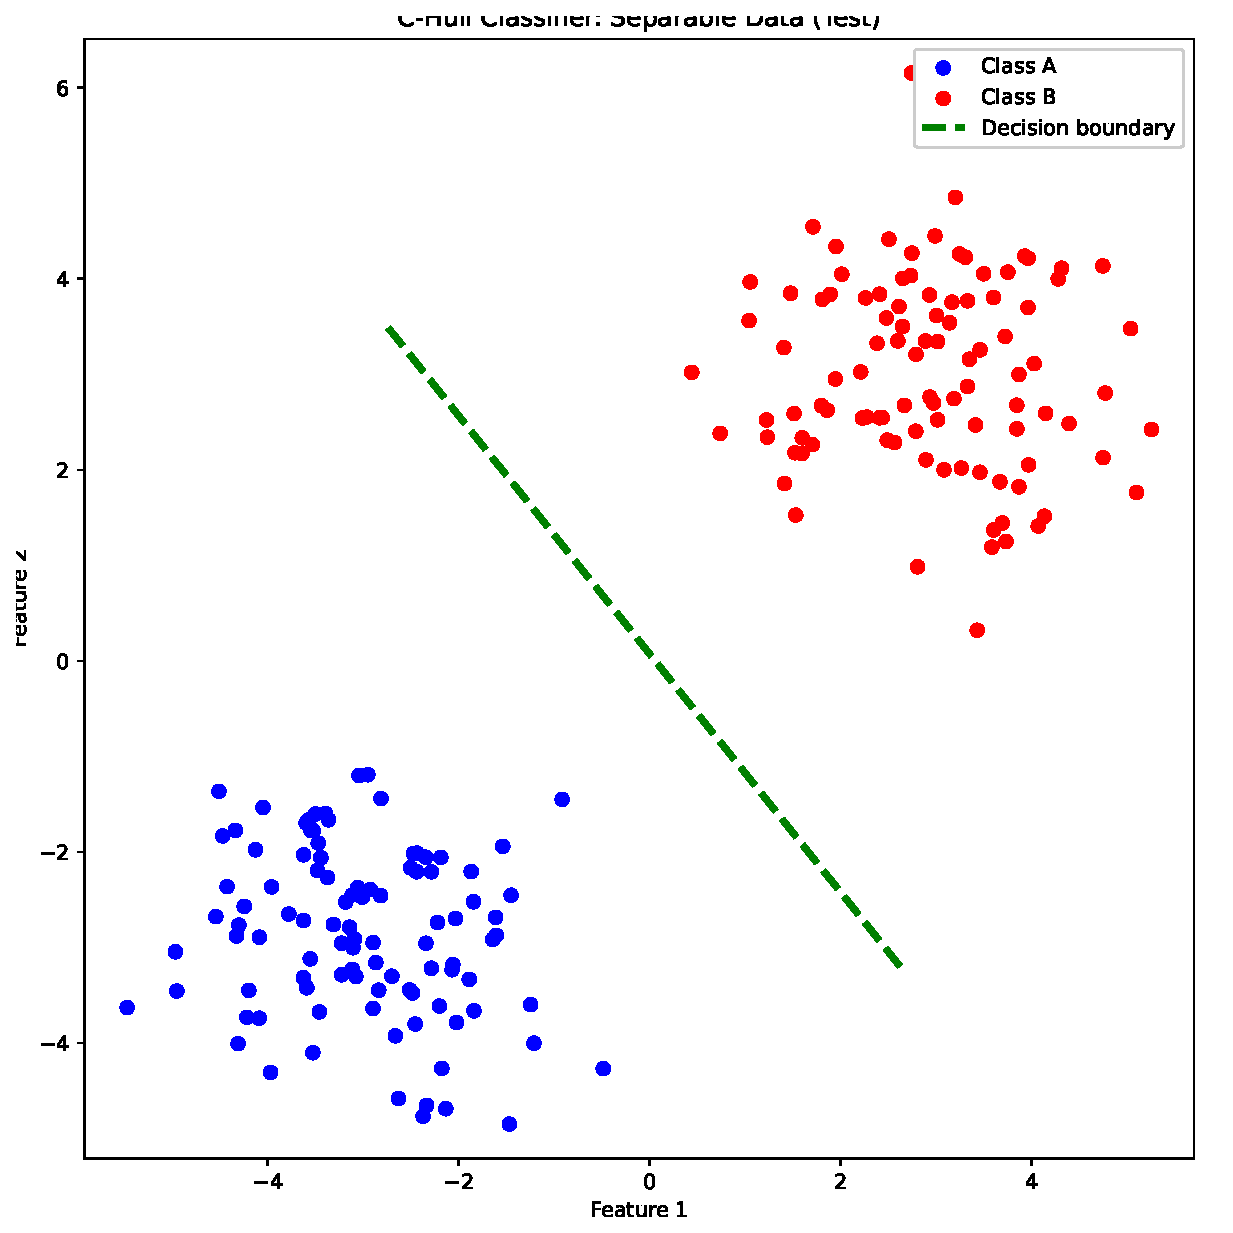
\includegraphics[width=\textwidth]{figures/school_work/ECE_569/HW_3/c-hull-separable-test.eps}
                \caption*{Figure 2: C-Hull Classifier, Separable Testing Data}
            \end{subfigure}

            % \caption{Training and Testing Data with Reduced C-Hull Classifier}
        \end{figure}
        After solving for a C-Hull classifier, the given test data is classified with 100\% accuracy.
        
        \newpage
        % question 1.b
        \part repeat the above for \qcr{train\_overlap.mat} and \qcr{test\_overlap.mat} using the reduced C-Hull:
        \begin{align*}
            \MIN{u, v} & ||Au - Bv ||_2^2 \\
            \subjectto & 1^Tu = 1, d1 \succeq u \succeq 0 \\
            & 1^Tv = 1, d1 \succeq v \succeq 0.
        \end{align*}
        Report the classification error on the testing data using an appropriate $d$.
        \begin{figure}[H]
            \centering

            \begin{subfigure}[b]{0.48\textwidth}
                \centering
                \includegraphics[width=\textwidth]{figures/school_work/ECE_569/HW_3/reduced-c-hull-overlapping-train.eps}
                \caption*{Figure 3: Reduced C-Hull Classifier, Overlapping Training Data}
            \end{subfigure}
            \hfill
            \begin{subfigure}[b]{0.48\textwidth}
                \centering
                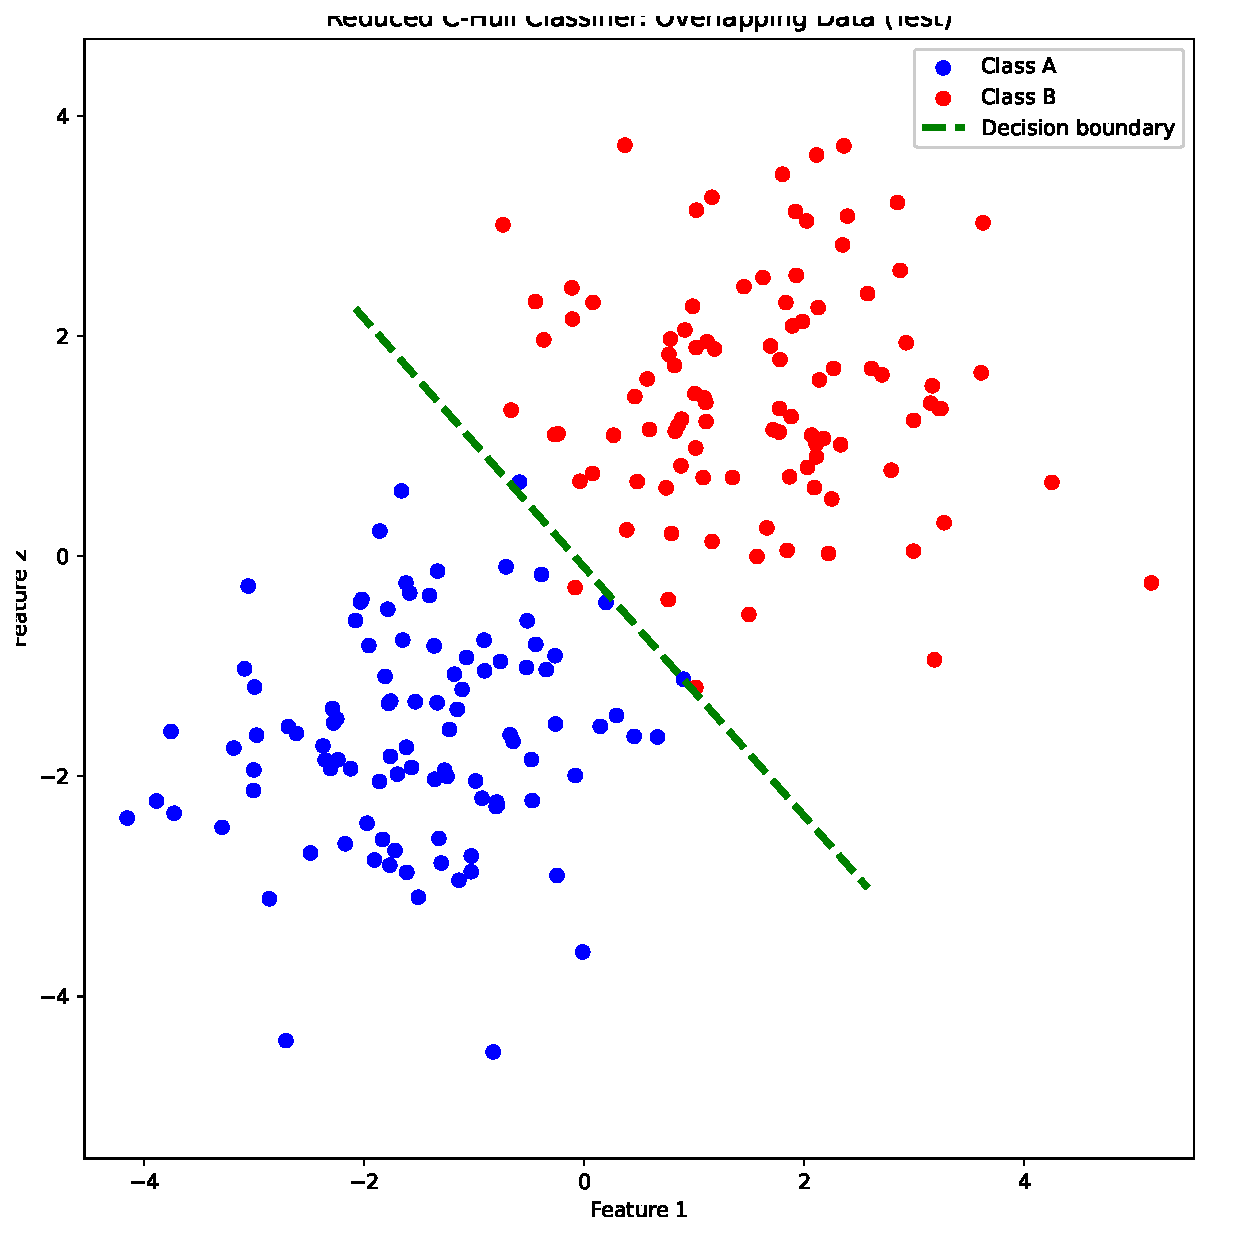
\includegraphics[width=\textwidth]{figures/school_work/ECE_569/HW_3/reduced-c-hull-overlapping-test.eps}
                \caption*{Figure 4: Reduced C-Hull Classifier, Overlapping Testing Data}
            \end{subfigure}

            % \caption{Training and Testing Data with Reduced C-Hull Classifier}
        \end{figure}
        After solving for a Reduced C-Hull classifier with $d = 0.75$ (admittedly arbitrary), an accuracy of 98.5\%
        is achieved on the test data.
    \end{parts}









    \newpage
    % question 2
    \question Under the same setting of Question 1, do the following:
    \begin{parts}
        % question 2.a
        \part Implement C-Hull and Reduced C-Hull using the projected gradient. Do the same visualization as in Question 1.
        \begin{figure}[H]
            \centering
            \begin{subfigure}[b]{0.48\textwidth}
                \centering
                \includegraphics[width=\textwidth]{figures/school_work/ECE_569/HW_3/pgd-c-hull-train.eps}
                \caption*{Figure 5: Projected Gradient (C-Hull), Separable Training Data}
            \end{subfigure}
            \hfill
            \begin{subfigure}[b]{0.48\textwidth}
                \centering
                \includegraphics[width=\textwidth]{figures/school_work/ECE_569/HW_3/pgd-c-hull-test.eps}
                \caption*{Figure 6: Projected Gradient (C-Hull), Separable Testing Data}
            \end{subfigure}
        \end{figure}
        \begin{figure}[H]
            \centering
            \begin{subfigure}[b]{0.48\textwidth}
                \centering
                \includegraphics[width=\textwidth]{figures/school_work/ECE_569/HW_3/pgd-reduced-c-hull-overlapping-train.eps}
                \caption*{Figure 7: Projected Gradient (Reduced C-Hull), Overlapping Training Data}
            \end{subfigure}
            \hfill
            \begin{subfigure}[b]{0.48\textwidth}
                \centering
                \includegraphics[width=\textwidth]{figures/school_work/ECE_569/HW_3/pgd-reduced-c-hull-overlapping-test.eps}
                \caption*{Figure 8: Projected Gradient (Reduced C-Hull), Overlapping Testing Data}
            \end{subfigure}
        \end{figure}
        Implementing projected gradient descent for the C-Hull yielded an accuracy of 100\% on the 
        separable test set. Projected gradient descent on reduced C-Hull yielded the same outcome as in question 1, with an
        accuracy of 98.5\% ($d = 0.75$) on the overlapping test set. The pseudo-code for the implementation for C-Hull and reduced C-Hull
        is provided in \qcr{q2\_pgd\_chull.py} and \qcr{q2\_pgd\_rchull.py} respectively.

        % question 2.b
        \part Repeat the above using Nesterov acceleration.
        \begin{figure}[H]
            \centering
            \begin{subfigure}[b]{0.48\textwidth}
                \centering
                \includegraphics[width=\textwidth]{figures/school_work/ECE_569/HW_3/nesterov-c-hull-separable-train.eps}
                \caption*{Figure 9: Nesterov Acceleration (C-Hull), Separable Training Data}
            \end{subfigure}
            \hfill
            \begin{subfigure}[b]{0.48\textwidth}
                \centering
                \includegraphics[width=\textwidth]{figures/school_work/ECE_569/HW_3/nesterov-c-hull-separable-test.eps}
                \caption*{Figure 10: Nesterov Acceleration (C-Hull), Separable Testing Data}
            \end{subfigure}
        \end{figure}
        \begin{figure}[H]
            \centering
            \begin{subfigure}[b]{0.48\textwidth}
                \centering
                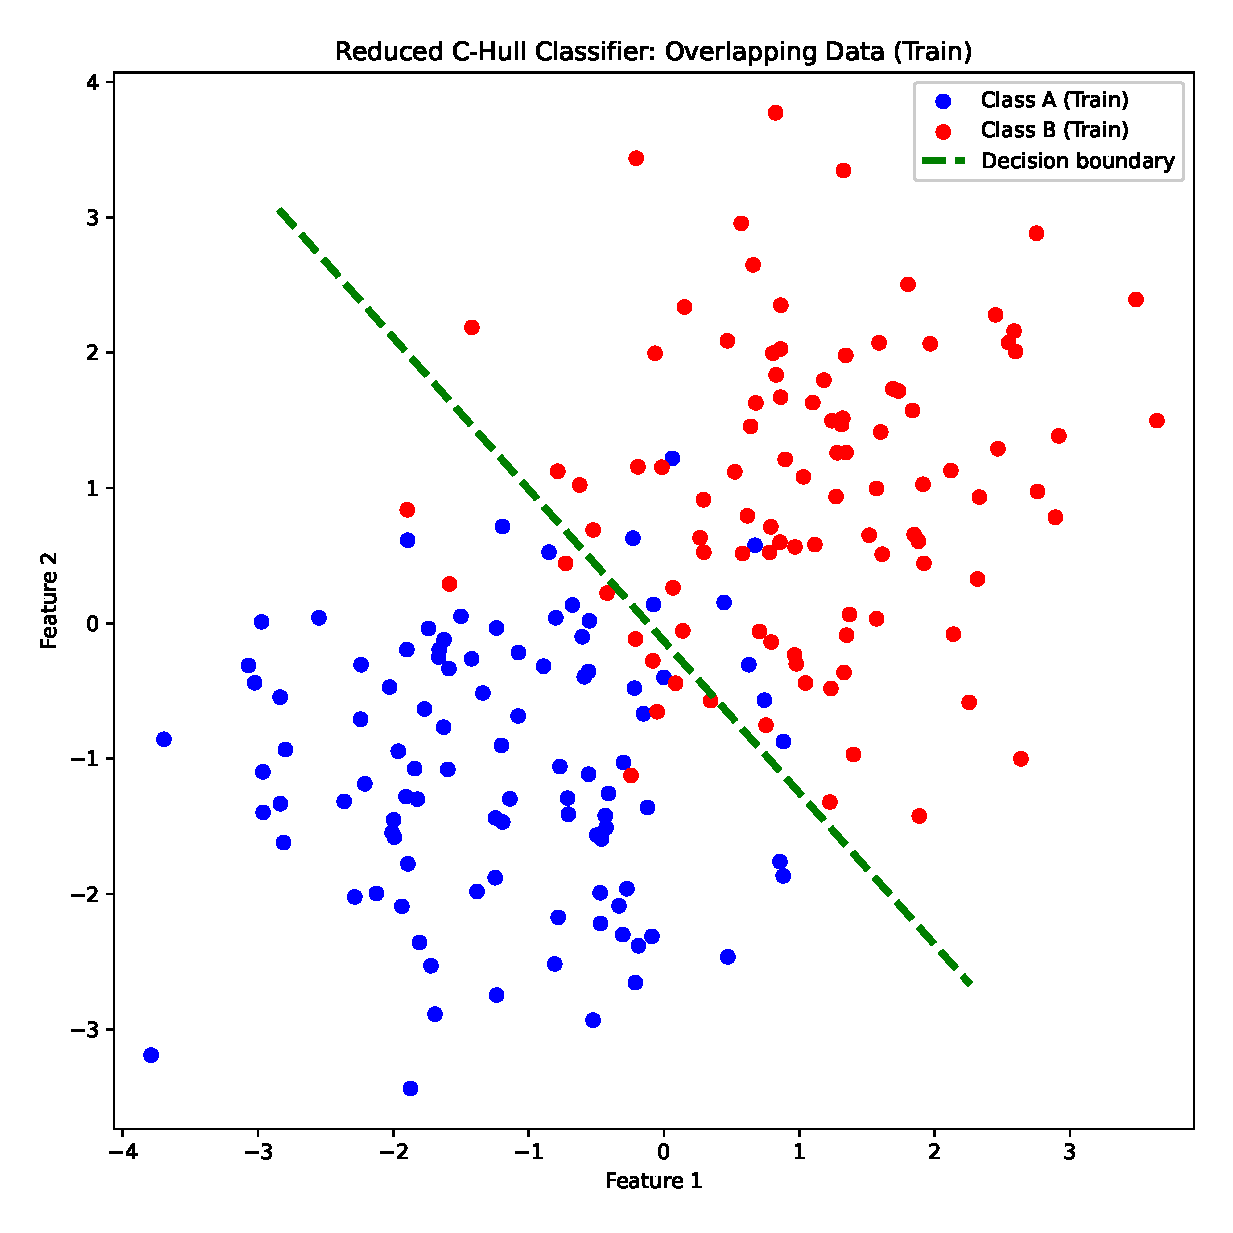
\includegraphics[width=\textwidth]{figures/school_work/ECE_569/HW_3/nesterov-reduced-c-hull-train.eps}
                \caption*{Figure 11: Nesterov Acceleration (Reduced C-Hull), Overlapping Training Data}
            \end{subfigure}
            \hfill
            \begin{subfigure}[b]{0.48\textwidth}
                \centering
                \includegraphics[width=\textwidth]{figures/school_work/ECE_569/HW_3/nesterov-reduced-c-hull-test.eps}
                \caption*{Figure 12: Nesterov Acceleration (Reduced C-Hull), Overlapping Testing Data}
            \end{subfigure}
        \end{figure}
        Implementing Nesterov acceleration for C-Hull gave a 100\% accuracy on the separable test data, and again the reduced C-Hull
        gave an accuracy of 98.5\% with $d = 0.75$. The pseudo-code for C-Hull and reduced C-Hull are in
        \qcr{q2\_nagd\_chull.py} and \qcr{q2\_nagd\_rchull.py} respectively.
    \end{parts}










    \newpage
    % question 3
    \question Under the same setting of Question 1, implement C-Hull and Reduced C-Hull using ADMM. Do the same visualization
    as in Question 1.
    \begin{figure}[H]
        \centering
        \begin{subfigure}[b]{0.48\textwidth}
            \centering
            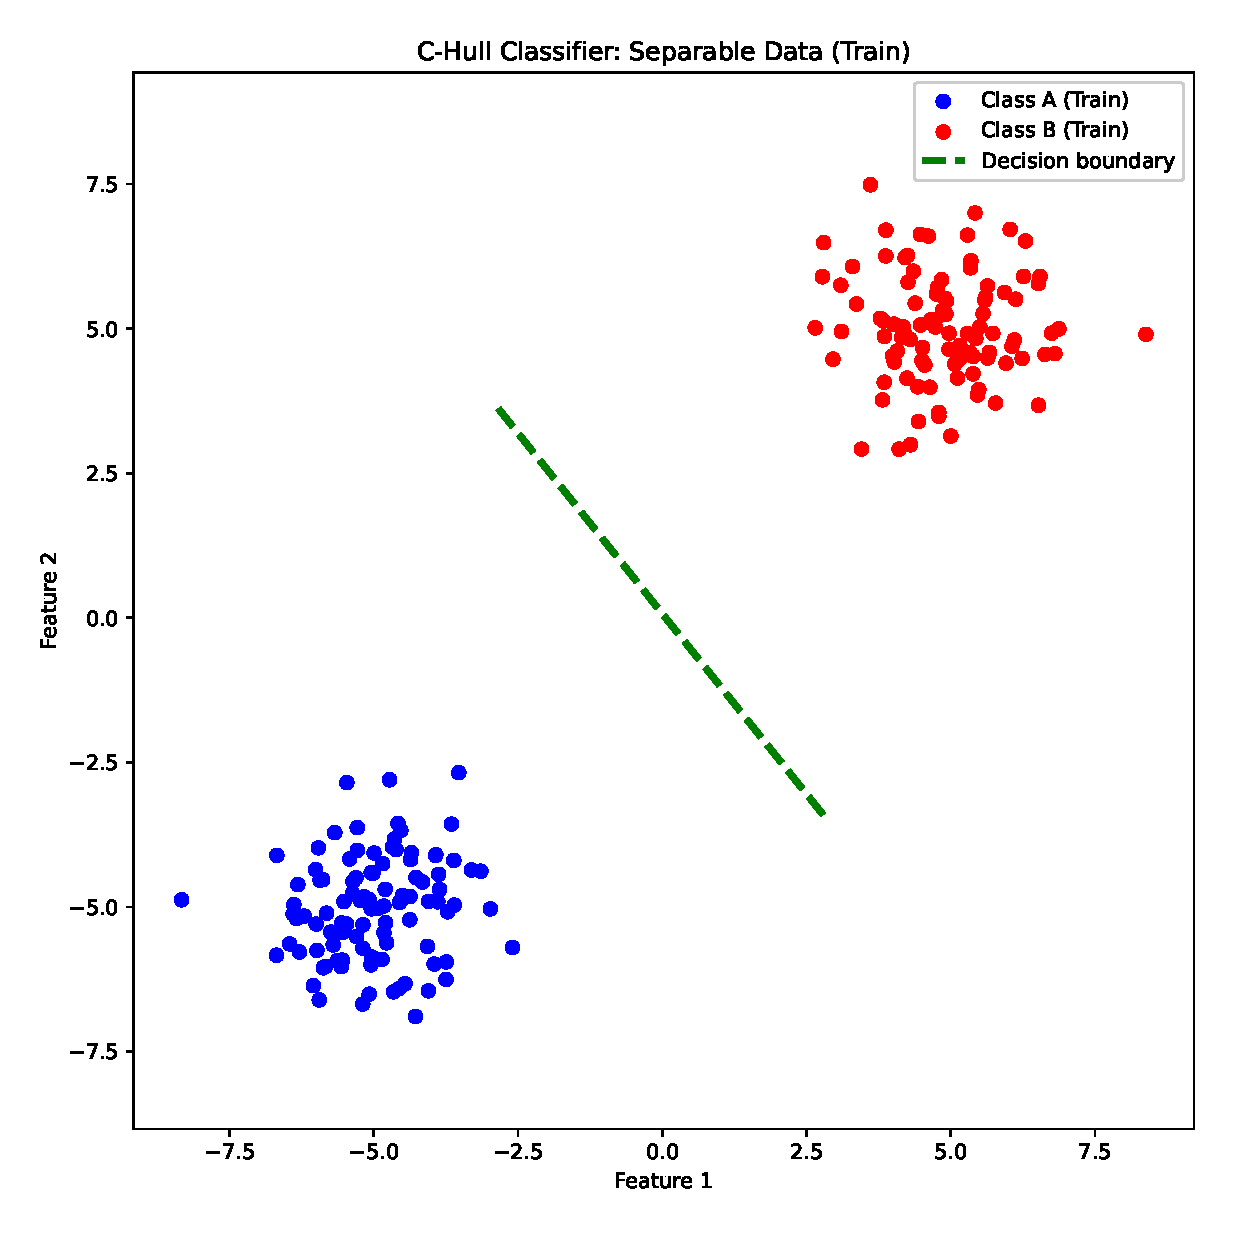
\includegraphics[width=\textwidth]{figures/school_work/ECE_569/HW_3/admm-c-hull-train.eps}
            \caption*{Figure 13: ADMM (C-Hull), Separable Training Data}
        \end{subfigure}
        \hfill
        \begin{subfigure}[b]{0.48\textwidth}
            \centering
            \includegraphics[width=\textwidth]{figures/school_work/ECE_569/HW_3/admm-c-hull-test.eps}
            \caption*{Figure 14: ADMM (C-Hull), Separable Testing Data}
        \end{subfigure}
    \end{figure}
    \begin{figure}[H]
        \centering
        \begin{subfigure}[b]{0.48\textwidth}
            \centering
            \includegraphics[width=\textwidth]{figures/school_work/ECE_569/HW_3/admm-reduced-c-hull-train.eps}
            \caption*{Figure 15: ADMM (Reduced C-Hull), Overlapping Training Data}
        \end{subfigure}
        \hfill
        \begin{subfigure}[b]{0.48\textwidth}
            \centering
            \includegraphics[width=\textwidth]{figures/school_work/ECE_569/HW_3/admm-reduced-c-hull-test.eps}
            \caption*{Figure 16: ADMM (Reduced C-Hull), Overlapping Testing Data}
        \end{subfigure}
    \end{figure}
    Using ADMM, implementing C-Hull gave a 100\% accuracy on the separable test data, and the reduced C-Hull
    gave an accuracy of 98.5\% with $d = 0.75$. The pseudo-code for C-Hull and reduced C-Hull are in
    \qcr{q3\_admm\_chull.py} and \qcr{q3\_admm\_rchull.py} respectively.














    \newpage
    % question 4
    \question Plot an Iteration vs Objective Value figure for the training process. Compare all the alogrithms that you implemented
    in this figure. In addition, plot a Time vs Objective Value figure using all the algorithms.
    
    DISCLAIMER: I am fairly confident the graphs are wrong, but I couldn't figure out how to fix them.


    % for q2.a projected gradient descent C-hull + reduced C-hull
    \begin{figure}[H]
        \centering
        \begin{subfigure}[b]{0.48\textwidth}
            \centering
            \includegraphics[width=\textwidth]{figures/school_work/ECE_569/HW_3/c-hull-time.png}
            \caption*{Figure 17: Time vs Objective Value (C-Hull)}
        \end{subfigure}
        \hfill
        \begin{subfigure}[b]{0.48\textwidth}
            \centering
            \includegraphics[width=\textwidth]{figures/school_work/ECE_569/HW_3/c-hull-iter.png}
            \caption*{Figure 18: Iteration (ms) vs Objective Value (C-Hull)}
        \end{subfigure}
    \end{figure}
    \begin{figure}[H]
        \centering
        \begin{subfigure}[b]{0.48\textwidth}
            \centering
            \includegraphics[width=\textwidth]{figures/school_work/ECE_569/HW_3/reduced-c-hull-time.png}
            \caption*{Figure 19: Time vs Objective Value (Reduced C-Hull)}
        \end{subfigure}
        \hfill
        \begin{subfigure}[b]{0.48\textwidth}
            \centering
            \includegraphics[width=\textwidth]{figures/school_work/ECE_569/HW_3/reduced-c-hull-iter.png}
            \caption*{Figure 20: Iteration (ms) vs Objective Value (Reduced C-Hull)}
        \end{subfigure}
    \end{figure}

    
\end{questions}


\end{document}